\documentclass{beamer}
\usepackage{graphicx}
\usepackage{amssymb,amsfonts,amsmath}
\usefonttheme[onlymath]{serif}
\usetheme{Madrid}

\title{Weekly Report}
\author{WU Zihan}
\date{\today}

\begin{document}

\maketitle

\section{Work Progress}

\begin{frame}
    \frametitle{Work Progress}
    \begin{itemize}
        \item Engaged in productive exchanges with Mehdi, sharing valuable data and code for our ongoing projects.
        \item Encountered challenges with the lack of `ground truth', raising considerations for its impact on our research publication validity.
        \item I think to co-cluster the positional data along the time is a better idea.
    \end{itemize}
\end{frame}

\begin{frame}
    \frametitle{Detailed Research in NLP}
    \begin{itemize}
        \item \textbf{Theme classification} Studies [1] [2] demonstrate the efficacy of two-way clustering of documents and words, facilitating refined document and topic categorization. Notable datasets include ``Yahoo\_K5'', ``Classic3\_3Odocs'', and ``Classic3\_150docs''.
        \item \textbf{Transfer Learning in NLP:} Research [3] highlights the role of co-clustering as a connecting bridge between labeled and unlabeled data, enabling effective topic classification beyond domain boundaries.
        \item \textbf{Information Dissemination:} Research [4] reveals the concept of overlapping co-clustering is leveraged for targeted information and news distribution, enhancing reach and relevance.
    \end{itemize}
    \textbf{References:} [1] Dhillon, 2001; [2] Dhillon et al., 2003; [3] Dai et al., 2007; [4] Sarkar \& Srivastava, 2014.
\end{frame}

\begin{frame}
    \frametitle{Accelarating Multimodal Learning based on Co-clustering}
    \begin{itemize}
        \item Recognized NLP's shift to multimodal models, merging diverse data types.
        \item Uncovered co-clustering's potential to enhance multimodal integration.
        \item Addressed training inefficiencies in contrastive learning.
        \item Suggested co-clustering to expedite training by reducing redundant computations.
    \end{itemize}
    % include clip.png
    \begin{figure}[htbp]
        \centering
        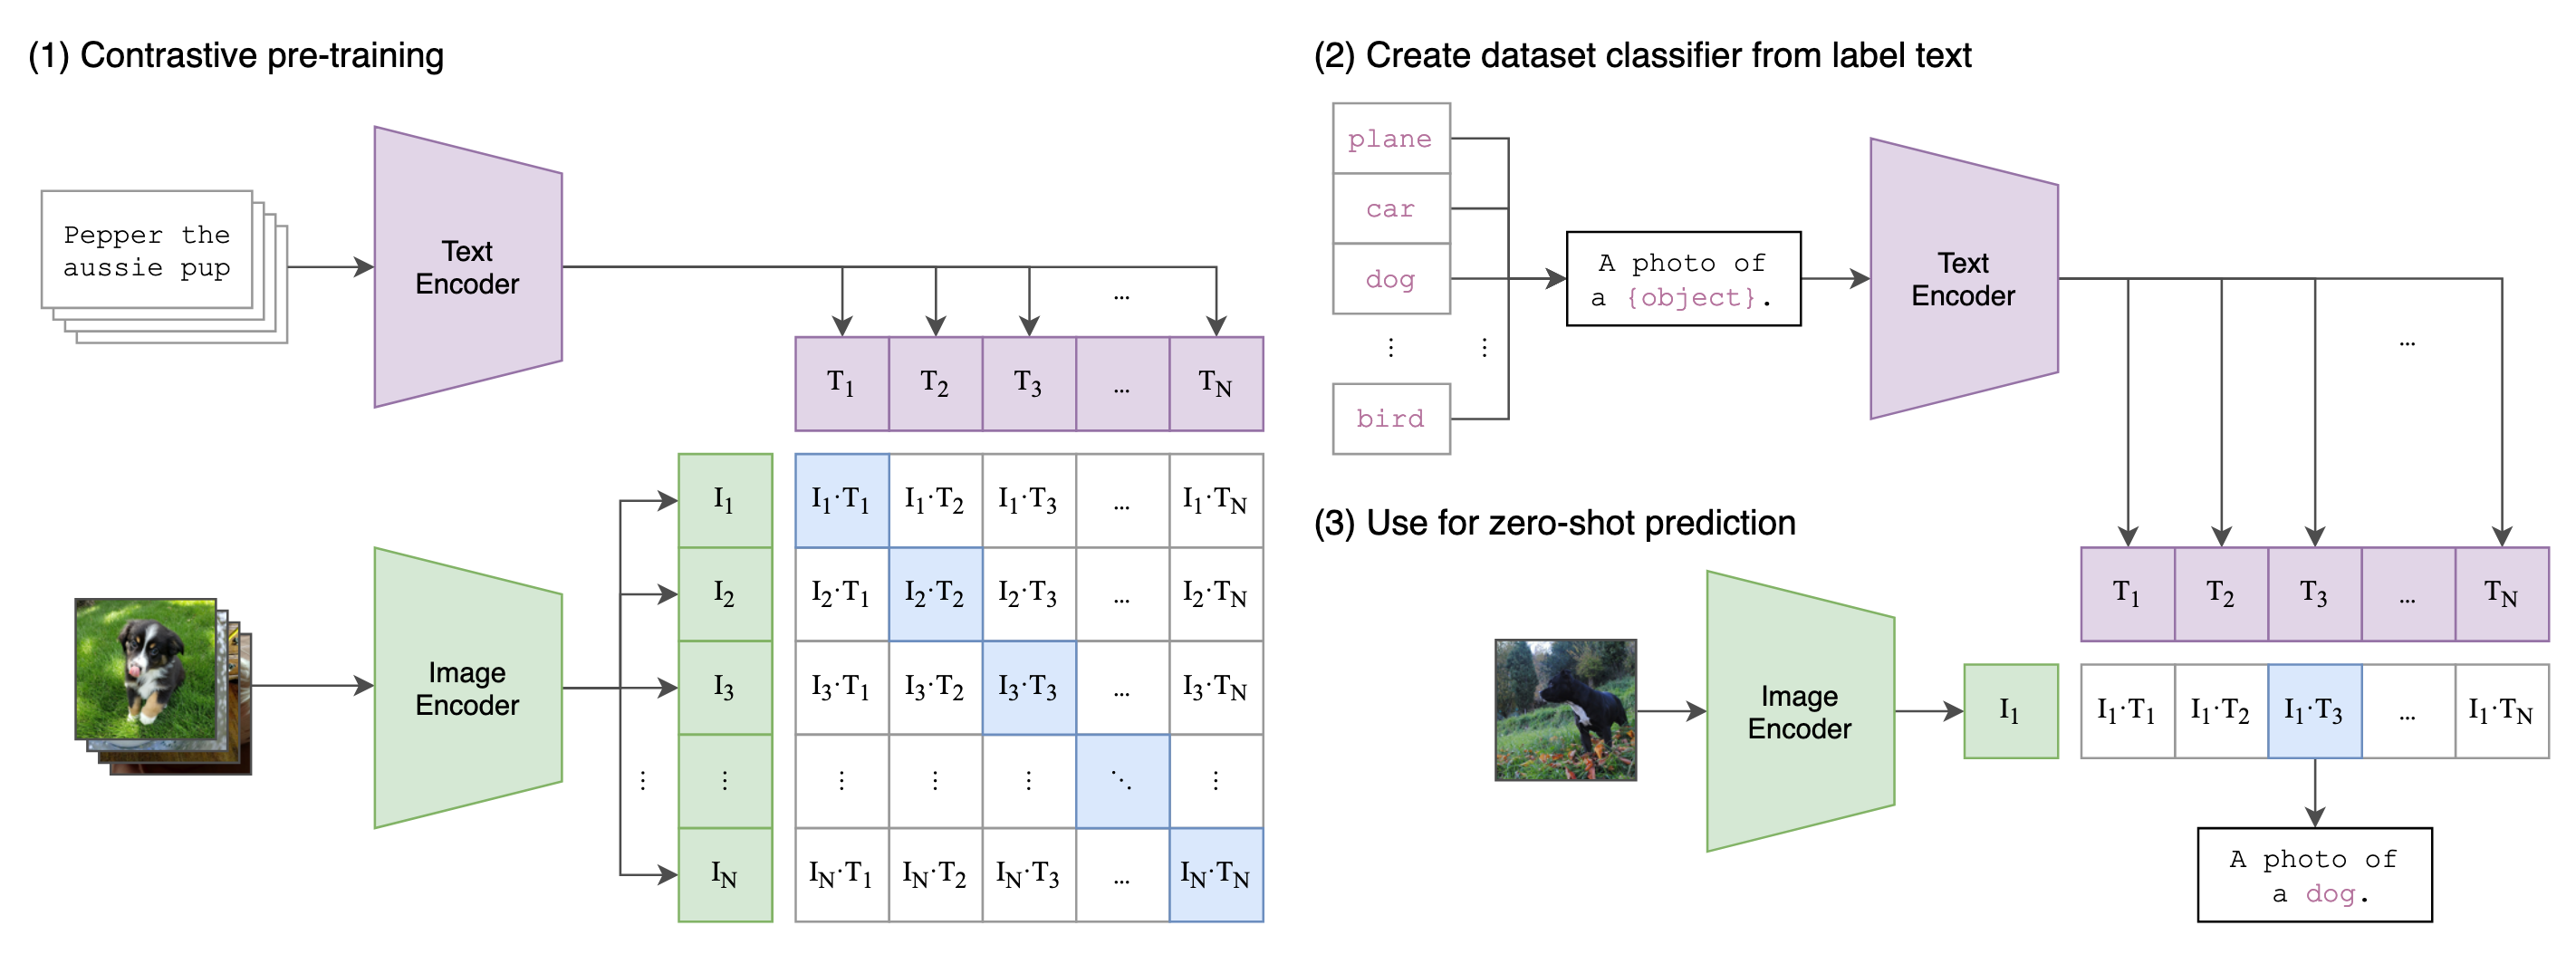
\includegraphics[width=0.7\textwidth]{clip.png}
        \caption{CLIP [1]'s training process.}
        % shrink vspace
        \vspace{-0.5cm}
    \end{figure}
    \textbf{Reference:} [1] Radford et al., 2021.
\end{frame}

\end{document}
